%
% File naacl2019.tex
%
%% Based on the style files for ACL 2018 and NAACL 2018, which were
%% Based on the style files for ACL-2015, with some improvements
%%  taken from the NAACL-2016 style
%% Based on the style files for ACL-2014, which were, in turn,
%% based on ACL-2013, ACL-2012, ACL-2011, ACL-2010, ACL-IJCNLP-2009,
%% EACL-2009, IJCNLP-2008...
%% Based on the style files for EACL 2006 by 
%%e.agirre@ehu.es or Sergi.Balari@uab.es
%% and that of ACL 08 by Joakim Nivre and Noah Smith

\documentclass[11pt,a4paper]{article}
\usepackage[hyperref]{emnlp-ijcnlp-2019}
\usepackage{times}
\usepackage{latexsym}

\usepackage{url}

%\aclfinalcopy % Uncomment this line for the final submission

%\setlength\titlebox{5cm}
% You can expand the titlebox if you need extra space
% to show all the authors. Please do not make the titlebox
% smaller than 5cm (the original size); we will check this
% in the camera-ready version and ask you to change it back.

\newcommand\BibTeX{B{\sc ib}\TeX}
\newcommand\confname{EMNLP-IJCNLP 2019}
\newcommand\conforg{SIGDAT}
\usepackage{amsmath,amsthm,amsfonts,amssymb,amscd}
\usepackage{graphicx}
\usepackage{multirow}
\usepackage{url}
\usepackage{float} 
\usepackage{tabularx}
\usepackage{xcolor}
\newtheorem{lemma}{Lemma}[section]
\newtheorem{theorem}{Theorem}[section]
\newtheorem{proposition}{Proposition}[section]
\newtheorem{definition}{Definition}[section]
\DeclareMathOperator*{\argmax}{argmax}
\DeclareMathOperator*{\argmin}{argmin}
\usepackage{algorithm}
\usepackage{algorithmic}
\usepackage[draft]{todo}
\floatname{algorithm}{Procedure}
\renewcommand{\algorithmicrequire}{\textbf{Input:}}
\renewcommand{\algorithmicensure}{\textbf{Output:}}
%\aclfinalcopy % Uncomment this line for the final submission
%\def\aclpaperid{***} %  Enter the acl Paper ID here

\newcommand{\fyTodo}[1]{\Todo[FY:]{\textcolor{orange}{#1}}}
\newcommand{\fyTodostar}[1]{\Todo*[FY:]{\textcolor{orange}{#1}}}
\newcommand{\fyDone}[1]{\done[FY]\Todo[FY:]{\textcolor{orange}{#1}}}
\newcommand{\fyDonestar}[1]{\done[FY]\Todo[FY:]{\textcolor{orange}{#1}}}

%\setlength\titlebox{5cm}
% You can expand the titlebox if you need extra space
% to show all the authors. Please do not make the titlebox
% smaller than 5cm (the original size); we will check this
% in the camera-ready version and ask you to change it back.

\title{Lexicalized Domain Representations for Neural Machine Translation}

\author{First Author \\% Minh Quang Pham\\
  Affiliation / Address line 1 \\
  Affiliation / Address line 2 \\
  Affiliation / Address line 3 \\
  {\tt email@domain} \\\And
  Second Author \\
  Affiliation / Address line 1 \\
  Affiliation / Address line 2 \\
  Affiliation / Address line 3 \\
  {\tt email@domain} \\}

\date{}

\begin{document}
\maketitle

\fyDone{s/naacl/EMNLP/g}
\fyDone{Too long, selfcontained, noref, rewrite}
\begin{abstract}
  Supervised machine translation works well when the train and test data are sampled from the same distribution.
  When this is not the case, \emph{adaptation} techniques help ensure that the knowledge learned from out-of-domain texts generalises to target domain sentences.
  We study here a related setting, \emph{multi-domain adaptation}, where the number of domains is potentially large and adapting separately to each domain would waste training resources.
  Our proposal transposes to neural machine translation the feature expansion technique of (Daum\'e III, 2007): it isolates domain-agnostic from domain-specific lexical representations, while sharing the rest of the network across domains.
  Our experiments use two neural architectures and two language pairs: they show that our approach, while remaining simple and computationally inexpensive, outperforms several strong baselines and delivers a multi-domain system that can successfully translate heterogeneous texts.

%   \fyTodo{Remove this}
%   THIS IS THE OLD ABSTRACT 
%   Fine-tuning a generic neural machine translation model to a certain domain usually degrade its performance on the other domains, thus it's very difficult to build a unique model which is best for all. Indeed, Catastrophic Forgetting, well-known problem in Machine Learning, states that standard backprogation neural network suffers a lot while there is a shift in training data distribution. However, Finetuning is very costly and unefficient in the industry therefore one best model is always desired. In this paper, we introduce an application of an old technique \cite{Daume07frustratingly} in Multi-Domain Neural Machine Translation. By defining general information encoding region and domain-specific encoding region in word embedding vector, we are able to seperate domain-related information flows in forward and backward propagation during training thus to
% mitigate the catastrophic interference happens during the training over different domains. Empirically, we achieved a unique model that has comparable score to finetuned models for every domains. Furthermore, our method is simple and could be applied to any architecture.
\end{abstract}

\section{Introduction \label{sec:introduction}}
% The problem
Owing to the development of flexible and powerful architectures based on neural networks \cite{Cho14properties,Bahdanau15learning,Ghering17convolutional,Vaswani17attention}, Machine Translation (MT) has made significant progresses over the past years, and constitute to date the standard for most production engines. The development of MT systems, be they neural or statistical, require very large parallel corpora consisting of millions of sentence pairs, a resource that only exist in very few application domains and language pairs. A lot of the recent research effort has thus focused on developping MT systems in restricted data conditions, for instance building multilingual MTs which enable zero-shot translation \cite{Firat16multiway,Ha16towards,Johnson17google}; %or even building systems without any parallel data \cite{Artetxe18unsupervised,Lample18unsupervised}.
Another important scenario for industrial MT is to adapt a neural system trained using parallel data in one domain to the peculiarity of other domains. Domain Adaption (DA) in MT is an old issue \cite{Foster07mixture,Axelrod11domain}, which comes in various guises, and for which a number of solutions have been studied. See the recent survey of \cite{Chu18asurvey} for neural MT. The typical setting is \emph{supervised adaptation}, where a (small) amount of data of the target domain of interest is used to fine-tune the parameters of a system trained on a large amount of texts in a source domain. We study here a different scenario, \emph{multi-domain adaptation} \cite{Sennrich13multidomain,Farajian17multidomain}, where we would like to use heterogenous data sources to train a unique system that would work well for all domains. This allows us to be both data efficient (all data is used to train all domains) and computationally efficient (we only train one system). %In our setting, we assume that the domain of test documents is known.

Multi-domain adaptation is conceptually close to multilingual MT, or more generally to multi-task learning \cite{Caruana97multitask}, and can be approached in a number of ways. We adapt here ideas of \citet{Daume07frustratingly} to neural MT.
% in an attempt to confine the differences between domains at the lexical level, while the rest of the parameters is shared between domains.
Our main hypothesis is that domains mostly differ at the lexical level, due to cross-domain polysemy, which motivates domain specific embeddings. By contrast, the deeper layers, which arguably model more abstract linguistic phenomena, are made shareable across domains. To this end, we design word embeddings containing a generic and several domain-specific regions. We experiment with three domains, two neural architectures and two language pairs and find that our technique yields effective multi-domain NMTs, outperforming several baselines. Our contribution is thus as follows:
%\begin{itemize}
%\item 
we implement the ideas of \cite{Daume07frustratingly} for two NMT architectures;
%\item 
we provide experimental evidence that suggest the effectiveness of this technique;
%\item 
our analysis of embeddings seems to confort our assumption that their variation across domain actually reflects a variation of senses.
%\end{itemize}
\fyDone{can we train in random order ? can we get away with catastrophic forgetting ?}
\fyDone{how to analyze the embeddings ? how can we test or claim ?}

\section{Lexicalized domain representations\label{sec:lexicalized_embeddings}}
\fyDone{Use meaningful titles throughout}

\subsection{Multi-domain machine translation \label{ssec:statement}}

Multi-domain machine translation is formalized as follows: we assume that our observations correspond to  domain-tagged sentence pairs $[(x,y),i]$, with $x$ in the source language, $y$ in the target language and $i$ a domain tag in $[1\dots d]$. We further assume a two-stage sampling process: first select a domain $i$ according to $p(i)$, then select a sentence pair according to a domain specific distribution $D_i$. Our objective is to find a set of parameters $\{\theta_1 \dots \theta_d \} \in \mathbb{R}^D \times \mathbb{R}^D \dots \times \mathbb{R}^D$ minimizing:
\begin{equation} \label{eq:loss}
\begin{split}
\sum_{i \in [1..d]} p(i) E_{(x,y) \sim D_{i}} [-log(p_{\theta}(y|x,i))]
\end{split}
\end{equation}
The training data for domain $i$ is denoted $C_i$.

A straightforward solution is to process each domain separately, computing the value $\theta_i^*$ that minimizes the empirical loss on the training corpus $C_i$. This strategy is only effective if we have sufficient training data for each domain; when this is not the case, some estimates $\theta_i^*$ may be far from their optimal value. \fyDone{Risk}
The alternative we consider here constraints each parameter $\theta_i$ to be made of two parts: $\theta_i = [\theta_s; \theta'_i]$ ($\theta_s \in R^{D_g}$) is shared across all domains, while the second part $\theta'_i \in \mathbb{R}^{D_i}$ is only used in domain $i$.
The parameter set is now much more constrained, yet we expect that tying parameters across domains will yield better estimates for $\theta_s$ due to a larger training corpus. In this setting, the optimization program defined by equation~\eqref{eq:loss} can no longer be performed separately for each training corpus.

\subsection{Lexicalized domain embeddings \label{ssec:lde}}

To actually implement this idea for NMT, we need to define the subset of parameters that will be common to all domain. We make the assumption that domain specificities can be confined to the lexical level, and define $\theta_s$ to contain all the network parameters, except for a subpart of the word embeddings. For each word $v$, the embedding vector $e(v)$ is thus decomposed as $e(v) = [e_g(v); e_1(v); \dots; e_d(v)]$, where $e_g(v)$ stores the generic lexical embedding, while $e_i(v)$ stores the subpart that is specific to domain $i$.
In our NMT architectures, the actual embedding layer composes these vectors linearly to generate the word embedding for domain $k$ according to:
\begin{align}
  \tilde{e}_k(v) =& M_g e_g(v) + \sum_{i \in [1,..,d]} M_i * e_i(v) * \delta(i=k) \nonumber \\
   & = M [e_g(v); e_1'(v,k) \dots; e_d'(v,k)], \label{eq:embedding}
\end{align}
where $\delta()$ is the Kronecker function, $M$ is the matrix made of blocks $M_g, M_1 \dots, M_d$, and $e_i'(v,k)$ is the masked embedding: $e_i'(v,k)= e_i(v) * \delta(i=k)$.  Making sure that the actual embedding do not contain any zero is important for the Transformer model, since the lexical representations are then summed to the positional encoding, which would undo the effect of domain masking, and propagate a gradient even to regions that should not be modified. With our design, we make sure that during backprogation, the matrix $M$ receives gradient $0$ at regions corresponding to deactivated regions in the word embedding. Those regions are also masked in forward step, thus do not interfere the training on the domain to which they are not assigned (see Figure~\ref{fig:network}).

\begin{figure}
  \center
  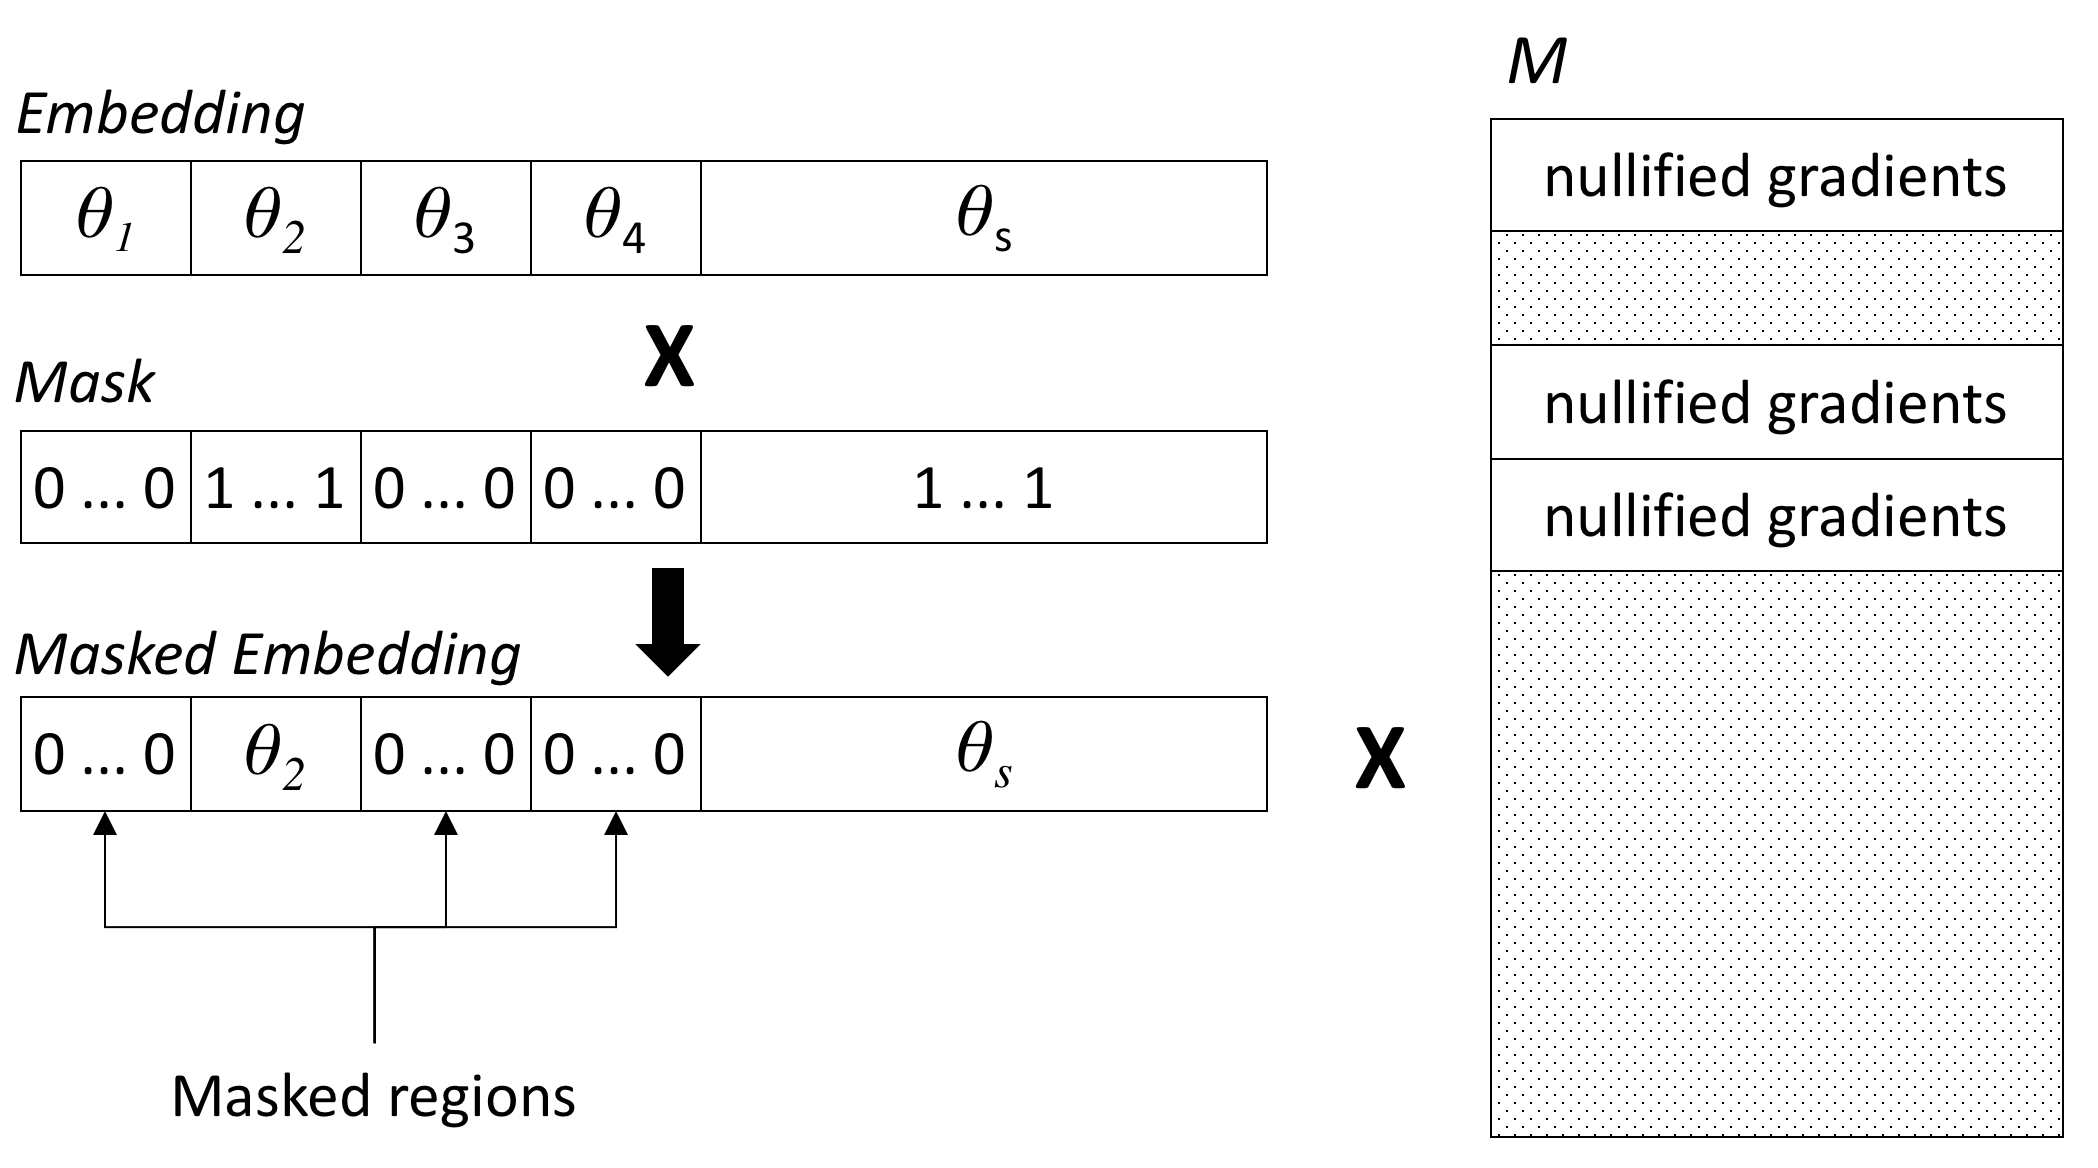
\includegraphics[width=0.48\textwidth]{embeddings}
  \caption{Lexicalized domain embeddings. When processing a sample from domain $2$, we only activate the corresponding parameter region ($\theta_2$) in the input embeddings; the remaining domain-specific parts are zeroed out, and do not receive any update. The generic part is always active, and is updated irrespective of the input domain.} 
  \label{fig:network}
\end{figure}

Our architecture is thus readily compatible with any NMT architecture, where we simply replace standard embedding layers the computation in equation~\ref{eq:embedding}. In our experiment, we consider both the attentional RNN architectures of \citet{Bahdanau15learning} and for Transformer architectures of \citet{Vaswani17attention}.

% Let $\tilde{x}_{t} = M * e_{t} = M_g e_g(t) + \displaystyle{\mathop{\sum}_{i \in [1,..,d]} M_i * e_i(t)}$ be the projection of word embedding where $e_{t}$ is word embedding of token $x_{t}$, M is projection matrix, $M_j \forall j \in [1...d]$ is row block corresponding to domain region $j$ (Transformer \cite{Vaswani17attention}, recurrent \cite{Bahdanau15learning})\\
% Assume the batch belongs to domain $i$, then $e_j(t) = 0$ $\forall j \neq i$,$\forall t$. 
% \begin{equation}
% \begin{split}
% \frac{\partial L(x,y)}{\partial M_j} &= \sum_{t}\frac{\partial L}{\partial \tilde{x}_t}(x_t) * \frac{\partial \tilde{x}_t}{\partial M_j} \\
% 								&= \sum_{t} \frac{\partial L}{\partial \tilde{x}_t}(x_t) * e_j(t)\\
% 									&=0
% \end{split} 
% \forall j \neq i
% \end{equation}

% The complex structure of State-of-the-art architecture Transformer \cite{Vaswani17attention} and popular recurrent network \cite{Bahdanau15learning} makes the implementation of sparse embedding non-obvious. Indeed, Transformer involve positional embedding and residual connections which are not homogeneous for domain-regions. Therefore, in our first implementation, we used an dense layer to fuse domain-region and generic region before applying positional embedding and residual connection. This implementation limits the finetuning effect at only word level.\\
% Furthermore, because word embeddings are involved in three parts of standard encoder-decoder structure, which are input of encoder, input of decoder and projection before softmax, we have 7 possibilities to apply sparse embedding. However, due to high memory cost, we only want to apply sparse embedding on the source side. \fyTodo{Explain this. Future work ?}


% %%% 
% \fyTodo{Use math for notation, label equations and such}
% \begin{definition}{Domain}
% \label{def:domain}
% A domain is probabilistic distribution of translation $(x,y)$ in a given corpora. Given corpora $C$, we denote $D(C)$ the domain of $C$.
% \end{definition}
% \fyTodo{We need more: the source, the target, etc}
% In machine translation, the loss function for training is:
% \begin{equation}\label{eq:1}
% \begin{split}
% E_{(x,y) \sim p_{rel}}[-log(p_{\theta}(y|x))] &= \\
% = E_{x \sim p_{rel}(x)}[KL(p_{rel}(y|x) & \mid p_{\theta}(y|x))] + \\
% + E_{x \sim p_{rel}} &[H(p_{rel}(y|x))]
% \end{split}
% \end{equation}.

% Where $p_{\theta}(y|x) = p(y|x,\theta)$ \\
% In this equation, the domain is $p_{rel}(x,y)$. In minimizing given objective \ref{eq:1}, one aims to approximate the objective domain $p_{rel}$. In inference, provided the model was trained on certain training data, the more likely test set is generated from domain of training data, the better performance.\\
% In general, a generic model is trained first with a mix of several corpora which belongs to different topics (e.g medical, banking, adminstration) whose the domain $p_{rel}$ is considered as a general domain, noted $p_{gen}$. Being trained with a general mixed corpora, the generic model is not usually good enough for translating by topic. In order to improve topical translation quality, specializing generic model is required. One usually finetunes the generic model by continue the training from initial value $\theta^*$, which was optimized on general domain, using corpora of interested topic. However, there is always a dramatical shift from generic domain $p_{gen}$ to specialization domain $p_{spec}$. Indeed, the translation $(x,y)$ could be very different in different topic. For instance, in financial document, to translate "security" into "titre financier" is more likely than to translate it into "securit\'e" but in IT document. Therefore, the shift from general domain containing these two corpora to one of them is not negligible. This shift usually leads to catastrophic forgetting in neural network using backpropagation \cite{McCloskey1989Catastrophic}. In effect, the finetuned model usually shows lower performance in translating sentences, which are less related to the finetuning topic, than generic model. 
% In order to conduct the model translating topic by topic, we might refer to conditional probability conditioned by topic $p(y|x,d)$. Given a set of training corpora, we assume that there are a limited d engendering topic, i.e, there are d corpora $C_i$ $i \in [1,..,d]$ representing d topical domains $D(C_i)$ respectively. We are then interested in approximating $p(y,x|i)$ for $i \in [1,..,d]$ and use $p(y|x,i)$ for the inference in topic $i$. From now, we formalize the multi-domain problem for machine translation in following equation
% \begin{equation} \label{eq:2}
% \begin{split}
% \theta^* = \argmin_{\theta} \displaystyle{\mathop{\sum}_{i \in [1..d]}} E_{(x,y) \sim D(C_{i})}[-log(p_{\theta}(y|x,i))]
% \end{split}
% \end{equation}
% It is obvious that
% \begin{equation} \label{eq:3}
% \begin{split}
% \argmin_{\theta} \displaystyle{\mathop{\sum}_{i \in [1..d]}} E_{(x,y) \sim D(C_{i})} &[-log(p_{\theta}(y|x,i))] \\
% \geq \displaystyle{\mathop{\sum}_{i \in [1..d]}} \argmin_{\theta} E_{(x,y) \sim D(C_{i})} &[-log(p_{\theta}(y|x,i))]
% \end{split}
% \end{equation}
% A trivial solution for the equation \ref{eq:2} is $\theta^* = (\theta^*_{0},...,\theta^*_{d})$ and $p_{(\theta_{0},...,\theta_d)}(y|x,i)$ is independent of $\theta_{j}$ $\forall j \neq i$, i.e, $\exists f:\Omega_i \times C(D_i) \rightarrow [0,1]: f_{\theta_i}(y,x) = p_{(\theta_{0},...,\theta_d)}(y|x,i)$ where $\Omega_i$ is set of all possible values of $\theta_i$. \\
% The trivial solution is not rather than ensemble of $d$ models specialized for one domain. However, we could reduce the seperation by using shared paramaters denoted $\theta_s$ then reformulate the model as following: \\
% $\theta^* = (\theta^*_{0},...,\theta^*_{d}, \theta_s^*)$ and $p_{(\theta_{0},...,\theta_d, \theta_s)}(y|x,i)$ is independent of $\theta_{j}$ $\forall j \neq i$, i.e, $\exists f:\Omega_i \times \Omega_s \times C(D_i) \rightarrow [0,1]: f_{\theta_i, \theta_s}(y,x) = p_{(\theta_{0},...,\theta_d, \theta_s)}(y|x,i)$ \\ $p_{(\theta_{0},...,\theta_d, \theta_s)}(y|x)$ is independent of $\theta_{j}$ $\forall j$ i.e, $\exists \bar{f}:\Omega_s \times C \rightarrow [0,1]: \bar{f}_{\theta_s}(y,x) = p_{(\theta_{0},...,\theta_d, \theta_s)}(y|x)$
% where $\Omega_i$ is set of all possible values of $\theta_i$ and $\Omega_s$ is set of all possible values of $\theta_s$. The optimization problem will become
% \begin{equation}
% \displaystyle{\mathop{\sum}_{i \in [1..d]}} \argmin_{\theta_{0},...,\theta_{d}, \theta_s} E_{(x,y) \sim D(C_{i})} [-log(p_{\theta_s,\theta_i}(y|x,i))]
% \end{equation}
% However, the couple $\theta_s^*$ and $\theta_i^*$ are hardly optimal $\forall i \in [1..d]$.\\
% Despite the fact that $\theta^* = (\theta^*_{0},...,\theta^*_{d}, \theta_s^*)$ is hardly achieved by backpropagation, we could attempt to optimize $\theta_s$:
% \begin{equation}
% \theta^*_{s} = \displaystyle{\mathop{\argmin}_{\theta_s}}E_{(x,y) \sim D(\displaystyle{\mathop{\cup}_{i \in [1,..,d]}}C_{i})}[-log(p_{\theta_s}(y|x))]
% \end{equation} 

% then optimize each $\theta_i$ (as additional factor used for fine-tuning the model to the domain $D(C_{i})$) the perplexity with respect to true distribution of domain
% \begin{equation}
% \theta^*_{i} = \displaystyle{\mathop{\argmin}_{\theta_i}}E_{(x,y) \sim D(C_{i})}[-log(p_{\theta_i,\theta^*_s}(y|x,i))]
% \end{equation} 
% Our first approach to multi-domain machine translation is to build such trivial solution by assigning different regions of word embedding vector to set of domain paramters $\theta_i$ and set of shared parameters $\theta_s$ while keep sharing other parameters between domains.


\section{Experiments \label{sec:experiments}}

\subsection{Domains and data \label{ssec:data}}

We experiment with two language pairs (English-French, English-German) and data originating from three domains, corresponding to texts from three European institutions: the European Parlement (EPPS) \cite{Koehn05europarl}, the European Medicines Agency (EMEA), and the European Central Bank (ECB) \cite{Tiedemann2009RANLP5}. We randomly split those corpora into training, validation and test sets (see statistics in Table~\ref{tab:Corpora}).\footnote{The EMEA dataset as distributed on the OPUS site contains many duplicates. We therefore report two numbers: the first is comparable to what has been published on earlier studies (eg.\ \cite{Zeng18multidomain}), the second one is obtained by making the test set entirely disjoint from the train.} The validation sets are used to chose the best model according to the average BLEU score \cite{Papineni02bleu}. Using internal test sets corresponds to somewhat ideal conditions; for contrast experiments, we also use supplementary test sets from three other domains: the official Khresmoi testset \cite{Khresmoi17test}, which is close to EMEA, News test 2014 \cite{Bojar14findings}, and IWSLT 2010 (Talk track) \cite{Paul10overview}. This enables us to evaluate the loss in performance when the test set is from a domain not seen in training.
% The model is also required to achieve comparable performance to generic model. To do so, we use newstest 2009 and IWSLT 2010 whose contain does not particularly belong to any domain.
\fyDone{Check which corpus are useful}
\begin{table}
  \centering
  \begin{tabular}{ *{4}{|r|}}
    \hline
    Corpus & Train & Dev & Test \\ \hline
    \multicolumn{4}{|l|}{En $\rightarrow$ Fr }\\
    \multicolumn{4}{|l|}{Vocabulary size - En: 30,165, Fr: 30,398}\\
    \hline
    EMEA  & 1,09M & 1000 & 1000$_{300}$\\
    ECB    & 0,19M & 1000 & 1000     \\
    EPPS   & 2,0M  & 1000 & 1000  \\ \hline \hline
    \multicolumn{4}{|l|}{En $\rightarrow$ De}\\
    \multicolumn{4}{|l|}{Vocabulary size -  En:30,159, De: 30,698}\\ \hline
    EMEA  & 1,11M & 1000 & 1000$_{300}$ \\
    ECB     &  0,11M & 1000 & 1000  \\
    EPPS   & 1,92M & 1000 & 1000 \\ \hline
\end{tabular}
\caption{Train and test corpora}
\label{tab:Corpora}
\end{table}
To reduce the number of lexical units and make our systems open-vocabulary, we apply Byte-Pair Encoding \cite{Sennrich16BPE} separately for each language with 30,000 merge operations. \fyDone{I need explanations here}

\subsection{Baselines \label{ssec:baselines}}
To validate our findings, we compared lexicalized domain embedding models with standard models using both attentional Recurrent Neural Networks (RNNs) \cite{Bahdanau15learning} and the recent Transformer architecture of \citet{Vaswani17attention}. Our baselines consist of generic models trained with a simple concatenation of all corpora (denoted \texttt{Mixed} in the tables below); models tuned separately on each domain using respectively (10000, 15000, 5000) iterations over in-domain data (denoted \texttt{ft(EMEA)}, \texttt{ft(EPPS)}, \texttt{ft(ECB)} below); models using domain tags as in \cite{Kobus17domaincontrol} (\texttt{DC} below); and finally the multi-domain model of \citet{Zeng18multidomain} (\texttt{WDCMT} below).\fyDone{Change names in tables}
For all models, we set the embeddings size equal to 512; the size of hidden layers is equal to 1024 for RNNs and 512 for Transformer. Other important configuration details are as follows:
\fyDone{Improve this}
%\begin{itemize}
%\item 
Transformer models use multi-head attention with 8 heads in each of the 6 layers; the inner feedforward layer contains 2048 cells; 
%  size of word embedding: 512; size of hidden layers: 512; size of inner feed forward layer: 2048; Multi-head: 8; number of layers: 6.
%\item 
RNN models use 1 layer on both sides: a bidirectional LSTM encoder and a unidirectional LSTM decoder with attention;
%  Attention Recurrent Neural Network: Bidirection LSTM encoder, unidirectional LSTM decoder, Luong Attention Mechanism, size of word embedding: 512; size of hidden layers: 1024; number of layers: 1
%\item 
The domain control systems are exactly as their baseline counterparts (RNN and Transformer), with an additional 2 cells encoding the domain on the input layer.\fyDone{Check This!}
  % C: size of domain embedding:2 ; same settings for both architecture: Transformer and Attention Recurrent Neural Network.
%\item 
The \texttt{WDCMT} system has one bidirectional Gated recurrent units (GRU) layer on the encoder side and one unidirectional conditional GRU layer on the decoder side; the dimension of ``domain'' layers is~300.
%\end{itemize}

To train NMT systems, we use Adam, with parameters $\beta_1=0.9$, $\beta_2 = 0.999$, $\alpha=0.0005$ for RNNs; with parameters $\beta_1=0.9$, $\beta_2= 0.98$, with Noam decay \cite{Vaswani17attention} for Transformer ($warmup\_steps=4000$). In all cases, we use a batch size of~128 and a dropout rate of 0.1 for all layers. 
All our systems are implemented in OpenNMT-tf\footnote{\url{https://github.com/OpenNMT/OpenNMT-tf}} \cite{Klein2017OpenNMT} except for WDCMT for which we use the authors' implementation.\footnote{\noindent\url{http://github.com/DeepLearnXMU/WDCNMT}}\fyDone{batch size}

\subsection{Implementing Lexicalized Domain Representations}\fyDone{Check acronym.}

\fyDone{Motivate the split - discuss experimentally embedding size}
In order to implement lexicalised domain representations (henceforth LDR), we split the embedding vector into four regions: 3 are domain specific and 1 is generic, with sizes $[8,8,8,488]$ respectively. %, a choice that will be discussed in Section~\ref{secc:region_size}. 
If a sentence originates from domain $i$, the domain specific regions for all domains $j \neq i$ will be zeroed out; while the rest of regions are activated (cf. Figure~\ref{fig:network}). We then use a dense layer of size~512 to fuse the region for the active domain and the ``generic'' region. Training is formalised in algorithm~\ref{alg:multidomain}.

\begin{algorithm}[h]
\caption{Multi-domain Training}
\label{alg:multidomain}
\begin{algorithmic}[1]
\REQUIRE {Corpora $C_i, i\in [1,..,d]$ for $d$ domains, Batch size $B$}%, Optimization algorithm $\operatorname{Opt}$}
\REPEAT 
\STATE{Randomly pick $i \in [1,..,d]$ w.r.t the multinomial distribution $[\frac{|C_i|}{\sum_{i\in [1,..,d]}|C_i|}]$.}
\STATE{Randomly pick $B$ sentences from $C_i$.}
\STATE{Activate only generic region to create generic batch, denoted $W_g$.}
% \STATE{Pass the generic embedding batch to a dense layer.}
\STATE{Compute gradient of $\theta_s$, $\frac{\partial L}{\partial \theta_s}$ using $W_g$.}
\STATE{Activate domain-specific and generic regions to create domain-specific batch $W_i$}
% \STATE{Pass $W_i$ to a dense layer}
\STATE{Compute gradient of domain-specific parameters $\theta_i$, $\frac{\partial L}{\partial \theta_i}$ using $W_d$.}
\STATE{Update parameters $\theta_s$ using $\frac{\partial L}{\partial \theta_s}(W_g)$ and $\theta_i$ using $\frac{\partial L}{\partial \theta_i}(W_i)$}
% $$ \theta_s = \theta_s - \operatorname{Opt}(\frac{\partial L}{\partial \theta_s}(W_g))$$ 
% $$ \theta_i = \theta_i - \operatorname{Opt} (\frac{\partial L}{\partial \theta_i}(W_i))$$}
\UNTIL{convergence}
\end{algorithmic}
\end{algorithm}

%In training, we use same optimization algorithm as for the baselines. 
%The same optimisation algorithm is always used.
Note that each iteration of algorithm \ref{alg:multidomain} uses 2~batches: a ``generic'' batch updating only the generic region; and a ``domain-specific'' batch updating just the domain-specific parameters. 
% Thus, we minimise two losses:
%This is because we wish to simultaneously minimize two losses:
% \begin{align*}
% \theta^*_{s}=&\displaystyle{\mathop{\argmin}_{\theta_s}}E_{(x,y) \sim D(\displaystyle{\mathop{\cup}_{i \in [1,..,d]}}C_{i})}[-log(p_{\theta_s}(y|x))] \\ 
%  \theta^*_{i}=&\displaystyle{\mathop{\argmin}_{\theta_i}}E_{(x,y) \sim D(C_{i})}[-log(p_{\theta_i,\theta^*_s}(y|x,i))]
% \end{align*} 

% We also take into account the problem of overfitting that could occur for small corpora. Indeed, real data are not always balanced for every domain. For instance, in our experiments, the size of corpora are very different where EPPS is largest with approximately 2 millions sentences, EMEA contains about 1 million sentences and ECB is the smallest with only 200 000 sentences for English French and 100 000 for English-German. If we train each corpora with same number of batches, ECB will be trained too oftenly, that easily leads to overfitting. Therefore, we select batches from each corpora with frequencies proportional to its size.
The batch selection procedure (step~2 of algorithm~\ref{alg:multidomain}) ensures that the number of examples seen in training of each domain follows the distribution of examples seen in the training data.
%each domain is represented according to its frequency in the training data. 
In our experiments, this means that sentences from the Europarl domain will be selected more frequently that the two other domains. In an attempt to build a more balanced training sample, we also consider an alternative selection procedure, where $i$ is selected according to  distribution $[\frac{\sqrt{|C_i|}}{\sum_{i\in [1,..,d]}\sqrt{|C_i|}}]$.
% \fyTodo{Refs on this ? or contrast ?}

\subsection{Results \label{ssec:results}}
% Discussion 1:
% \begin{itemize}
% \item transformer better than RNN
% \item Fine tuning is the best strategy - but subject to catastrophic
% \item Sparse better than joint - better than domain control
% \item Across th board / language \& architecture - always good for EMEA , less good for EPPS, varying for ECB
% \item better ? than domain control ? WMCD ?
% \end{itemize}

% Discussion 2:
% \begin{itemize}
% \item Sparse 1 > Sparse 2
% \item out of domain better than Mixed
% \item Sparse 3 ??
% \item ajouter Sparse 4
% \end{itemize}

Our main results are summarized respectively in Table~\ref{tab:results-trsf} for the Transformer systems and Table~\ref{tab:results-rnn} for the RNN systems, where we report BLEU scores \cite{Papineni02bleu} computed after detokenization.\footnote{As explained above, we consistently report two numbers when testing with EMEA, except for the fine-tuning scenarios when tuning on ECB and EPPS.} % \fyTodo{Footnote for missing numbers}.

We first concentrate on the left part of these tables, where we analyze the performance for the three domains of interest. A first series of observations is that Transformer is consistently better than RNN, and that fine-tuning on a domain-specific corpus, when applicable, is almost the best way to optimize the performance on that domain.\footnote{This is not so clear for the EPPS, where fine-tuning does not seem to help.}  Note that fine-tuning will however yield a marked (even sometimes catastrophic, eg.\ for the EMEA-tuned Transformer system) decrease in performance for the other domains. 

For these test sets, our proposal (\texttt{LDR}$_{oracle}$) is consistently better that the mix-domain strategy, with gains that range from very large (for EMEA and ECB) to unsignificant (for EPPS in most conditions). This means that our architecture is somehow able to compensate for the data unbalance and to raise the performance of the multi-domain system close to the best (fine-tuned) system in each domain. We even observe rare cases where the \texttt{LDR}$_{oracle}$ system outperforms fine-tuning (eg.\ Transformer en:de in the EMEA domain). \texttt{LDR}$_{oracle}$ is also better than Domain Control in three conditions out of four, \texttt{DC} being seemingly a better choice for the RNN than for the Transformer architecture. The comparison with the \texttt{WDCMT} model is less favourable for our RNN systems, which are arguably much simpler.\footnote{The direct comparison with WDCMT is difficult as the implementation differs in many ways from our RNN: a different framework, different cell types,
  % (LSTMs vs. conditional GRUs),
  etc.} \fyDone{More on this.}
As expected, ignoring the domain label yields a drop in performance for the two fallback strategies considered in this study. The first, \texttt{LDR}$_{generic}$, only uses the generic part of the embeddings. The second, \texttt{LDR}$_{pred}$, resorts to automatically predicted domain labels\footnote{Our domain classifier uses a bi-LSTM RNN encoder, followed by a simple softmax layer. Its precision on a development set are higher than 95\%.}
\fyDone{Explain how} Note that this decrease is however quite limited (and hardly significant for \texttt{LDR}$_{pred}$), showing that our architecture is quite robust to noisy labels. Even in the worst case scenario where all domain tags are intently wrong (\texttt{LDR}$_{wrong}$), we see that the generic part still ensures a satisfying level of performance. A last contrast is with \texttt{LDR}$_{oracle}^{0.5}$ where we change the distribution of training sentences to decrease the weight of EPPS data and increase the number of ECB samples. As a result, we see a small decrease for EMEA and EPPS, and a large boost for ECB. This shows that our technique can be used in conjunction to other well known strategies for performing domain adaptation. 

% \fyTodo{Comment V2 from Minh}

The right parts of Tables~\ref{tab:results-trsf} and \ref{tab:results-rnn} report performance on test sets for new domains not seen in training. Khresmoi texts, which are extracted from summaries of medical articles are assumed to be from the same domain as EMEA data; for the other two test sets, we assume no domain and only use the generic part of the embeddings. Here, we see that our best system \texttt{LDR}$_{oracle}$ is slightly lagging behind the \texttt{Mixed} baselines (the difference ranges from unsignificant to one Bleu point), which can be attributed to larger useful (generic) embeddings in the \texttt{Mixed} setting. Here again, we see that using the sole generic part makes the system robust with respect to unknown or misleading domain tags. We finally outline that our approach outperforms DC for these test sets (were we have to commit to a predicted domain tag), and even outperforms WDCMT (for German-English). This might be due to the fact that WDCMT has no built-in mechanism to ignore, as we do in the \texttt{LDR}$_{generic}$ systems, the possibly misleading predicted domain information.

\begin{table*}[!h]
\begin{center}
\scalebox{1.0}{
\begin{tabular}{|l|ccc|ccc||c|}
\hline
Model & EMEA & EPPS & ECB & Khresmoi & NewsTest2014 & IWSLT2010 & Avg. \\
\hline
\multicolumn{8}{l}{} \\[-9pt]  
\multicolumn{8}{l}{English$\rightarrow$French} \\
\hline
$Mixed$ & 67.69$_{47.60}$ & 37.50 & 53.49 & 34.86 & 28.56 & 25.70 & 41.3\\
\hline
$\mathtt{FT} (EMEA)$ & 76.77$_{49.43}$ & 17.16 & 11.99 & 29.58 & 11.64 & 11.10 & 26.37 \\
$\mathtt{FT} (EPPS)$  & 20.86 & 37.04 & 24.53 & 31.86 & 28.33 & 11.10 & 25.62 \\
$\mathtt{FT} (ECB)$   & 26.93 & 27.09 & 56.52 & 22.04 & 17.51 & 13.99 &  27.35\\
\hline
$\mathtt{DC}$ & 67.87$_{45.42}$ & 37.31 & 54.14 & 33.63 & 26.52 & 24.81 & 40.71\\
\hline
$\mathtt{LDR}_{oracle}$   & 74.26$_{49.90}$ & 37.67 & 54.07 & 33.85 & 28.11 & 25.70 & 42.28\\
$\mathtt{LDR}_{oracle}^{0.5}$   & 74.95$_{49.38}$ & 37.35 & 55.91 & 33.57 & 27.59 & 25.27 & 42.44\\
$\mathtt{LDR}_{generic}$ & 73.97$_{49.54}$ & 37.81 & 53.67 & 34.17 & 28.11 & 25.70 & 42.24 \\
$\mathtt{LDR}_{pred}$ & 74.29 $_{49.84}$ & 37.73 & 54.01 & 33.34 & 28.32 & 26 & 42.28\\
$\mathtt{LDR}_{wrong}$ & 72.95$_{49.78}$ & 37.62 & 53.35 & - & - & - & - \\
  \hline
\multicolumn{8}{l}{} \\[-9pt]
\multicolumn{8}{l}{English $\rightarrow$German} \\
\hline
$Mixed$ & 64.57$_{42.99}$ & 26.47 & 68.67 & 21.77 & 17.04 & 18.85 &36.23 \\
\hline
$\mathtt{FT} (EMEA)$ & 68.35$_{42.97}$ & 17.02 & 32.87 & 21.15 & 11.21 & 13.49 & 27.35\\
$\mathtt{FT} (EPPS)$ & 36.19 & 26.29 & 40.71 & 19.67 & 16.47 & 19.24 & 31.42\\
$\mathtt{FT} (ECB)$  & 24.72 & 18.36 & 74.05 & 11.31  & 10.8 & 11.00 & 25\\
\hline
$\mathtt{DC}$ & 63.48$_{42.98}$ & 26.27 & 66.95 & 21.45 & 16.45 & 18.78 & 35.56\\
\hline
$\mathtt{LDR}_{oracle}$ & 70.9$_{46.12}$ & 26.30 & 68.9 & 21.42 & 16.57 & 18.82 & 37.15\\
$\mathtt{LDR}_{oracle}^{0.5}$ & 71.31$_{45.23}$ & 25.98 & 73.74 & 21.6 & 16.37 & 19.2 & 38.03\\
$\mathtt{LDR}_{generic}$ & 70.86$_{45.60}$ & 26.14 & 68.59 & 21.95 & 16.57 & 18.82 & 37.14\\
$\mathtt{LDR}_{pred}$ & 70.89$_{46.12}$ & 26.53 & 68.63 & 21.45 & 16.61 & 19.07 & 32.2 \\
$\mathtt{LDR}_{wrong}$ & 69.51$_{43.50}$ & 26.31 & 66.86 & - & - & - & - \\
\hline
\end{tabular}
} %scalebox
\end{center}
\caption{BPE-detokenized BLEU scores for the Transformer systems \label{tab:results-trsf}}
\end{table*}

\begin{table*}[!h]
\begin{center}
\scalebox{1.0}{
\begin{tabular}{|l|ccc|ccc||c|}
\hline
Model & EMEA & EPPS & ECB & Khresmoi & NewsTest2014 & IWSLT2010 & Avg. \\
\hline
\multicolumn{8}{l}{} \\[-9pt]
\multicolumn{8}{l}{English$\rightarrow$French} \\
\hline
$Mixed$               & 65.42$_{45.11}$ & 34.7 & 51.38 & 29.27 & 22.21 & 21.63 &37.43 \\
\hline
$\mathtt{FT} (EMEA)$  & 72.06$_{47.33}$ & 18.62 & 16.78 & 25.88 & 10.94 & 5.73 & 20 \\
$\mathtt{FT} (EPPS)$    & 35.47 $ $ & 34.61 & 39.56 & 27.11 & 21.85 & 20.61 & 29.87 \\
$\mathtt{FT} (ECB)$     & 21.93 $ $ & 22.6 & 51.53 & 14.74 & 12.10 & 10.47 & 22.23 \\
\hline
$\mathtt{DC}$                   & 68.26 $_{43.76}$ & 35.13 & 50.09 & 27.86 & 20.95 & 21.16 & 37.24\\
 \hline
$\mathtt{WDCMT}$           & 68.76 $_{45.29}$ & 35.71 & 52.75 & 32.03 & 24.63 & 23.28 & 38.97 \\
\hline
$\mathtt{LDR}_{oracle}$   & 71.73 $_{46.30}$ & 35.21 & 50.91 & 29.62 & 23.00 & 20.96 & 38.57\\
$\mathtt{LDR}_{oracle}^{0.5}$   & 71.7$_{46.41}$ & 34.24& 52.37 & 29.21 & 22.7& 20.69 & 38.48\\
$\mathtt{LDR}_{generic}$ & 70.59 $_{46.37}$ & 35.22 & 49.68 & 29.51 & 23.00 & 20.96 & 38.16\\
$\mathtt{LDR}_{pred}$        & 72.76 $_{46.35}$ & 35.1 & 50.38 & 30.02 & 23.28 & 21.32 & 38.81\\
$\mathtt{LDR}_{wrong}$   & 62.1 $_{43.29}$ & 34.17 & 48.79 &  - & - & - & - \\
\hline
\multicolumn{8}{l}{} \\[-9pt]
\multicolumn{8}{l}{English$\rightarrow$German} \\
\hline
$Mixed$               & 57.37 $_{37.94}$ & 23.1 & 63.54 & 17.39 & 11.51 & 14.29 & 31.2\\
\hline
$\mathtt{FT} (EMEA)$  & 65.64$_{44.71}$ & 12.36 & 15.93 & 15.38 & 6.22 & 7.6  & 20.53\\
$\mathtt{FT} (EPPS)$   & 24.90 $ $ & 22.98 & 26.26 & 13.55 & 11.33 & 14.32 & 18.89 \\
$\mathtt{FT} (ECB)$    & 41.8 $ $ & 15.97 & 71.07 & 10.77 & 7.66 & 8.07 & 25.89\\
\hline
$\mathtt{DC}$                      & 62.53 $_{39.25}$ & 23.74 & 65.71 & 16.88 & 11.15 & 14.97 & 32.50\\
\hline
$\mathtt{WDCMT}$ & 64.05 $_{38.54}$ & 22.82 & 67.00 & 15.94 & 11.45 & 13.66 & 32.49\\
\hline
$\mathtt{LDR}_{oracle}$   & 63.43 $_{40.04}$ & 22.66 & 64.40 & 16.99 & 11.45 & 14.26 & 32.2\\
$\mathtt{LDR}_{oracle}^{0.5}$   & 63.27 $_{38.16}$ & 21.83 & 69.55 & 15.7 & 11.32 & 13.98 & 32.6\\
$\mathtt{LDR}_{generic}$ & 63.27 $_{39.75}$ & 22.62 & 63.70 & 17.26 & 11.45 & 14.26 & 32.1\\
$\mathtt{LDR}_{pred}$        & 63.17 $_{39.92}$ & 22.51 & 64 & 15.94 & 11.32 & 14.27 & 31.87\\
$\mathtt{LDR}_{wrong}$   & 56.84 $_{37.05}$ & 22.06 & 61.66 & - & - & - & - \\
\hline
\end{tabular}
} %scalebox
\end{center}
\caption{BPE-detokenized BLEU scores for the RNN systems\label{tab:results-rnn}}
\end{table*}
% \clearfloat

\section{Complementary experiments\label{sec:Discussion}}
% \subsection{Sparse's performance}
% First, we analyze the performance of models on inner test sets which are created by randomly splited from same corpora as training set. The 4 table show remarquable improvement 6 points BLEU in average in EMEA translation which is comparable with finetuned model. In all most the cases, Sparse model has slightly higher score on EPPS test and ECB test than mixed and finetuned models. Sparse model also achieve comparable scores with Domain Control and WDCMT in average. In considering the score of finetuned model on out-of-domain test sets, we observed a fast catastrophic forgetting while the out-of-domain scores drop dramatically compared to mixed model. Taking into account the average score on 3 inner test sets, Sparse achieved far better score than all finetuned models. \\
% Secondly, we compare performance of models on IWSLT test 2010 and newstest 2014 which are more general than inner test sets. On these test sets, mixed, Sparse has approximately same score in Transformer and are a little better than Domain Control while in Recurrent Net Work architecture, WDCMT is better than mixed, Sparse and Domain Control for English -French pair. We also noted a quick fall of performance in finetuned model.

\subsection{Balancing generic and domain-specific representations\label{secc:region_size}}

An important practical question concerns the balance between the generic and the domain-specific part of the embeddings. In the limit where the domain specific part is very small, we should recover the performance of the \texttt{Mixed} system; conversely, we expect to see a less effective sharing of data across domains by increasing the domain-specific regions. Table~\ref{tab:embedding-size} reports the result of  a series of experiments for the Transformer architecture (English-French) with varying domain-specific sizes allocating between 4 and 64 cells for domain-specific information, and the complement to 512 for the generic part. The differences are overall quite small in our experimental setting, where the training data is relatively limited and does not require to use a large embedding size. We therefore decided to allocate $8$~cells for the domain specific part. This suggests that we could easily accomodate more domains with the same architecture, and even reserve some regions to handle supplementary incoming training data.  
% \fyTodo{Easily accomodate more domains}
\fyDone{Given the ways embeddings are computed, why not add more domains, and test robustness agains data presentation order ?}

\begin{table*}[!h]
\begin{center}
\scalebox{1.0}{
\begin{tabular}{|l|ccc|ccc|}
\hline
$LDR$ & EMEA & EPPS & ECB & Khresmoi & NewsTest2014 & IWSLT2010 \\
\hline
\multicolumn{7}{l}{English$\rightarrow$French} \\
\hline
 size=4   & 74.65 $_{49.61}$ & 37.42 & 54.49 & 33.68 & 28.03 & 25.28 \\
 size=8   & 74.26 $_{49.90}$ & 37.67 & 54.07 & 33.85 & 28.11 & 25.70 \\
 size=16 & 74.15 $_{49.10}$ & 37.78 & 54.56 & 33.40 & 28.10 & 25.33 \\
 size=32 & 75.10 $_{48.61}$ & 37.64 & 54.29 & 33.20 & 27.99 & 25.44 \\
 size=64 & 74.5 $_{50.17}$ & 37.27 & 54.5 & 33.26 & 27.95 & 25.65 \\
\hline
\end{tabular}
} %scalebox
\end{center}
\caption{BPE-detokenized BLEU scores for the Transformer architecture for varying domain-specific embedding sizes \label{tab:embedding-size}}
\end{table*}

\subsection{Analysis of Word Embeddings \label{ssec:word_embeddings}}
One of our main assumptions is that the difference between domains can be confined at the lexical level, warranting our decision to specialize lexical representations for each domain, while the remaining part of the network is shared across domains. Linguistically, this assumption relates to the classical ``one sense per collocation'' \cite{Yarowsky93onesense} and corresponds to the fact that in many cases, polysemy corresponds to variation of use across domain. In its weaker form, it allows us to assume that all occurrences of a given form in a given domain correspond to the same sense and share the same representation; the same form occuring in different domains is allowed to have one distinct embedding per domain, which may help capture polysemy and lexical ambiguity in translation. 

To check the validity of this hypothesis, we performed the following analysis of embeddings learned with the multi-domain Transformer system for English:French. For each unit\footnote{In this study, we work with BPE units, not words, meaning that in many cases we observe the variation of use of word parts. As we work with a large inventory, many of these units correspond to actual words, and we focus on these in our comments. We also restrict our analysis to words that occur at least 30 times in each domain, to ensure that each domain-specific region is updated during training.} in our English dictionary, we compute the $k$ nearest neighbours for each domain $i \in [1\dots{}d]$, where the distance between unit $u$ and $v$ for domain $i$ is the cosine distance in the corresponding embedding space, ie.\ assuming that the actual embedding of $v$ for domain $d$ is $e(v,i) = M_ge_g(u) + M_de_i(v)$ (cf.\ equation~\eqref{eq:embedding}). This process yields $d$ lists of $k$ nearest neighbours. The size of their intersection should then be a sign of a variation of use across domains; conversely, an identical set of neighbours across domains should reflect the stability of word use. Table~\ref{tab:embeddings} list the 10 units with the smaller (respectively larger) intersection (we use $k=10$ and $d=3$). 

\begin{table}
  \centering
  \begin{tabularx}{1.0\linewidth}{c|c}
    Polysemic ``words'' & Monosemic ``words'' \\ \hline
     ases (0) &               obtain (10) \\       
     impairment (1) &     virtually (10) \\    
     convenience (1) &    represent (10) \\    
     oring (1) &              safety (10) \\       
     ums (1) &               defence (10) \\      
     turnover (1) &         coordinated (10) \\  
     occurrence (1) &     handling (10) \\     
     tent (2) &               July (10) \\         
     ture (2) &               previous (10) \\     
     mation (2) &           better (10) \\ \hline
  \end{tabularx}
  \caption{Analyzing the variation of embeddings across domains. Each word or subword is listed with the size of the intersection (between 0 and 10).}
  \label{tab:embeddings}
\end{table}

Let us first consider the full words in the left column of Table~\ref{tab:embeddings}. The case of \emph{impairment} is pretty clear, occuring in EMEA mostly in terms such as ``hepatic impairment'' or ``renal impairment'', and translating into French as \textsl{insuffisance}. In ECB, its collocate are quite different, and impairment often occurs in terms such as ``cost subject to impairments'' (French: \emph{co\^ut soumis \`a des r\'eductions de valeur}). Likewise, ``convenience'' seems to have its general meaning (``for convenience'') in EMEA, but appears in ECB in the specific context of ``convenience credit card'' (French \textsl{carte de cr\' edit \`a remboursement diff\'er\'e}). We finally see the same phenomena with ``turnover'', which is consistently translated with its economic meaning (French \textsl{chiffre d'affaire}) in ECB and EPPS, but whose collocates in EMEA ("bone turnover", ``hepatic turnover'') are associated with the idea of the cell renewall process, yielding translations such as \textsl{remodelage osseux} in French. Subword units can be analysed in the same ways: ``ums'', for instance, appears in words such as ``gums'', ``serums'', ``vacuums''  in EMEA; in ECB, ``ums'' is mostly the suffix of ``maximums'', ``minimums'', or ``premiums''; EPPS finally contains a more diverse set of ``-ums'' ending words (``stadium'', ``forum'', equilibrium'', etc). 

Let us now consider the list of putative monosemic words (on the right part of Table~\ref{tab:embeddings}), ie.\ words for which the nearest neighbors are the same in all domains, contains mostly words for which we do not expect much variation in translation: adjective (``previous'', ``better''), adverbs (``virtually``), generic verbs (``handling'', ``coordinated''), etc; and the list of words having a constant set of neighbors also contains prepositions (``at'', ``in''), auxiliary (``been'') etc.  

% \begin{table}
%   \centering
%   \begin{tabular}{*{4}{|r|}}
%     \hline
%     Domain & Word & Neighbor & Cosinus distance \\ \hline
%     \multirow{5}{*}{EMEA} & \multirow{5}{*}{joint} 
%     & Joint & 0.371 \\  
%     &  & jointly & 0.545 \\
%     &  & artic- & 0.605 \\
%     &  & joints & 0.607 \\
% 	&  & collective & 0.609 \\
% 	\hline
% 	\multirow{5}{*}{EPPS} & \multirow{5}{*}{joint} 
% 	& Joint & 0.365 \\
% 	& & jointly & 0.497 \\
% 	& & join- & 0.606 \\
% 	& & common & 0.607 \\
% 	& & collective & 0.626 \\
% 	& & artic- & 0.633\\
% 	\hline
% 	\multirow{5}{*}{ECB} & \multirow{5}{*}{joint}
% 	& Joint & 0.423 \\
% 	& & jointly & 0.467 \\
% 	& & common & 0.601 \\
% 	& & together & 0.632 \\
% 	& & artic- & 0.663 \\
% 	& & coordinated & 0.668 \\
% \end{tabular}
% \caption{Corpora}
% \label{tab:Polysemy}
% \end{table}

\section{Related Work \label{sec:related_work}}
\fyDone{Add standard labels to sections}
\fyDone{Related work goes last}
\fyDone{Compare also to Peng 2017}

% Multi-domain Machine Translation has largely interested NLP community by its promising applications in industry and its relation to fundamental problems in theory. Researchers have proposed a large range of techniques from Data centric methods to Model centric methods \cite{Chu18asurvey}.\\ Data centric category attempts to collect related-domain data from large existing in-domain corpora. The methods in this category can be listed as following:
% \fyTodo{Organize refs}

% \begin{itemize}
% \item score relatedness of sentences to the target domain by Language Model \cite{Moore2010selection,Axelrod2011domain,Duh2013selection}.
% \item generating pseudo parallel data \cite{Utiyama2003measure,Wang2016connecting,Wang2014neural}
% \end{itemize}
% On the other hand, model-centric approaches focus on NMT models that are specialized for domain adaptation. The novelty can be among following features:
% \begin{itemize}
% \item Trainining objective\cite{Luong2015SNMT,Sennrich2016Mono,Wang17instance,Chen17costweighting,Miceli2017Regularize,Zhang18sentence}
% \item Architecture \cite{Gulcehre2016monolingual,Zhang16topicinformed,Kobus17domaincontrol,Britz2017mixing,Biao2017CARENMT,Britz2017mixing,Thompson18freezing,Michel2018extreme}.
% \item The decoding algorithm \cite{Gulcehre2016monolingual,Khayrallah2017lattice}
% \end{itemize}
% Beside these works \fyTodo{Works= oeuvres d'art}, we could also consider works in other tasks such as sequence labeling tasks \cite{Daume07frustratingly}; learning multiple visual domains \cite{Rebuffi2017Visual}.

%% HERE
Domain adaptation (DA) is a vexing problem in NLP, which appears in a wide range of practical situations and data scenarios (eg.\ supervised vs. unsupervised adaptation), and  has been thoroughly  studied from a number of perspectives, ranging from theoretical analysis to more applied work, and for which many solutions have been proposed. The literature of DA for Machine Translation reflects this diversity and typically distinguishes data-based approaches from model-based approaches \cite{Chu2017comparison,Chu18asurvey}.

The most common adaptation scenario uses (mostly) out-of-domain data in training, while testing on a low-resource in-domain set of texts. In this setting, \emph{data-based approaches} aim to bias the distribution of the train (out-of-domain) data towards matching that of the target domain, using data selection techniques \cite{Moore2010selection,Axelrod2011domain,Duh2013selection}, or generating adapted pseudo-parallel data through back-translation  \cite{Utiyama2003measure,Wang2014neural,Wang2016connecting,Sennrich2016Mono}. \emph{Model-centric approaches} build domain-adapted models by combining (eg.\ with mixture weights) multiple data sources or multiple systems \cite{Foster07mixture,Wang17instance}, or by biasing the training objective towards the desired domain using in-domain adaptation data \cite{Luong2015SNMT,Freitag2016FastDA,Chen17costweighting}. Another approach worth mentioning integrates domain information (for instance a domain language model) in the decoding algorithm \cite{Gulcehre2016monolingual}.

Our scenario is a bit different as we aim to train a unique system that will work well for several domains. This corresponds to a practical scenario in the industry, where one would like to maintain one single multi-domain engine, trained on all the available (heteregeneous) sources of data. Our primary source of inspiration is the proposal of \citet{Daume07frustratingly} who proposes to use several copies of the same features (one ``generic'' shared across domains, and one for each domain), letting the training adjust their respective weights. This work has been reanalyzed in a Bayesian framework in \cite{Finkel09hierarchical}, and revisited notably in \cite{Chang10necessity}. Following up on \cite{Yang15unified}, the recent proposals of \cite{Peng17multitask} apply the same idea with neural architectures, using domain specific masking to zero out the parameters modeling domains irrelevant to the current input sentence. Compared to our work, these techniques are used in deep layers of the network and applied to sequence labelling tasks.

The multi-domain scenario in NMT has been studied in a number of recent works. \citet{Farajian17multidomain} learn a generic system and propose to dynamically adapt the network weights in an unsupervised manner using a small sample of training data that resembles the test data, an idea already explored in \cite{Sennrich13multidomain}. Their main contribution is to propose an a method to relate the amount of adaptation of the network parameters to the similarity between the adaptation sample and the test sentence: the higher the similarity, the more agressive the adaptation.

By analogy with the proposal of \citet{Johnson17google} for multilingual NMT, \citet{Kobus17domaincontrol} and \citet{Chu18multilingual} separately propose to extend the representation of the source text with a domain tag. Our model also modifies input representations, but allows each source word to have a domain-specific representation, thereby improving training of the shared parts of the network.\fyDone{Talk about target embeddings somewhere.} 

Similarly to our approach, \cite{Zeng18multidomain} attempts to separate on the encoder side domain-specific representation from generic representations in two different sub-networks, where generic versus domain-specific representations automatically emerge from two adversarial networks. The decoder side can thus attend separately to these two representations to generate its output. In this approach, the shared and domain-specific part kept separated in the deeper layers of the network, whereas we try to localize the differences between domains at the lexical level, based on a much cheaper computational architecture. Another trait of this proposal is the ability to automatically infer domain information for test sentences; as we have shown, our architecture can also effectively accomodate sentences lacking domain information.

% creates in the encoder Domain-specific gate $g^r_i$and Domain-shared gate $g^s_i$ which are generated from domain-specific and domain-shared semantic representations of source sentence $E_r(x)$ and $E_s(x)$ respectively and which select information from units of hidden states $h_i$ by elementwise product $h^r_i = g^r_i \odot h_i$; $h^s_i = g^s_i \odot h_i$. $h^r_i$ and $h^s_i$ will be fed to Domain-specific and Domain-shared attentional mechanisms respectively. While introducing new features in the architecture, \cite{Zeng18multidomain} also introduces new loss function which is sum of word-level weighted MT loss and losses of Domain-classifier in source side and target side; Adversarial Domain-classifier in source side. The authors have very good approach to seperate Domain-shared information flow and Domain-specify information flow and to determine their contributions to the inference thus mitigate the catastrophic interference occuring in training with backpropagation.

% The problem is recently investigated by several interesting works presented in EMNLP 2018 such as \cite{Platanios18contextual}; \cite{Zeng18multidomain} creates in the encoder Domain-specific gate $g^r_i$and Domain-shared gate $g^s_i$ which are generated from domain-specific and domain-shared semantic representations of source sentence $E_r(x)$ and $E_s(x)$ respectively and which select information from units of hidden states $h_i$ by elementwise product $h^r_i = g^r_i \odot h_i$; $h^s_i = g^s_i \odot h_i$. $h^r_i$ and $h^s_i$ will be fed to Domain-specific and Domain-shared attentional mechanisms respectively. While introducing new features in the architecture, \cite{Zeng18multidomain} also introduces new loss function which is sum of word-level weighted MT loss and losses of Domain-classifier in source side and target side; Adversarial Domain-classifier in source side. The authors have very good approach to seperate Domain-shared information flow and Domain-specify information flow and to determine their contributions to the inference thus mitigate the catastrophic interference occuring in training with backpropagation

% Platanios is multilingual !!
% \cite{Platanios18contextual} has other idea to circumvent the catastrophic interference. They supposed that parameters of each domain specialized model could be generated from a universal parameter-generator. By introducing domain embedding (or language embedding in the original paper), they could conduct domain related error in backpropagation toward domain embedding thus mitigates catastrophic interference between domains during training.

% Compared to \cite{Platanios18contextual}, our sparse embedding is a bit similar to the idea. However, our method gives much more free degree for domain embedding since we give each word a domain region while the author uses only one vector domain embedding for each parameter set(encoder, decoder).

% Compared to the work of \cite{Zeng18multidomain}, our approach is much simpler and
% more generic, since sparse embedding can be implemented for every neural architecture while domain-specific gate and domain-shared gate can only be applied for recurrent architectures. However, during inference, the model of \cite{Zeng18multidomain} can infer the domain that is the closest to the input sentence and that will be used in special gates; while our method needs to know in which domain the inference is executed. To circumvent this disadvantage, we could use a domain classifier or simply use only the generic region. For more detail, the reader could refer to the Section \ref{sec:sparse_embeddings}.

\section{Conclusions}
In this paper, we have presented a new technique for multi-domain machine translation, adapting to two common NMT architectures the ``frustratingly easy'' idea of \cite{Daume07frustratingly}. Our experiments have shown that for both architecture and for two language pairs, our multi-domain models improve over several baselines of the literature, and that it is robust to noise in domain labels. In our future work, we intend to develop this work so as to make the architecture more self-configurable and able to adapt the size of the domain-specific regions depending upon the actual variation of use across domains; we also would like to find ways to make the architecture able to integrate new domains in a dynamic fashion, as this is an important requirement in industrial systems.

% \fyTodo{natural continuations: bayesian version ? linear combination of specialized engines ? go beyond words; learn the projection matrix at the word level; other ?}

%\section*{Acknowledgments}
% \fyTodo{Homegenize refs - urls, addresses, etc}
\bibliography{emnlp-ijcnlp-2019}
\bibliographystyle{acl_natbib}
\end{document}
